\documentclass[10pt]{article}
\usepackage{ctex}
\usepackage{geometry}
\geometry{a4paper,scale=0.8}
\usepackage[T1]{fontenc}
\usepackage{mathptmx}
\usepackage{amsmath}
\usepackage{fancyhdr}
\pagestyle{fancy}
\fancyhead[L]{上海交通大学计算机学院}
\fancyhead[R]{NIS4307\ 人工智能导论（A类）}
\fancyfoot[C]{\thepage}
\newcommand{\code}[1]{\allowbreak\texttt{#1}\allowbreak}
\usepackage{titlesec}
\titlespacing{\paragraph}{0pt}{1ex plus 0ex minus .2ex}{1em}
\usepackage{enumitem}
\setlist[itemize]{topsep=0pt, itemsep=0pt, partopsep=0pt, parsep=0pt}
\setlist[enumerate]{topsep=0pt, itemsep=0pt, partopsep=0pt, parsep=0pt}
\usepackage{url}
\usepackage[colorlinks=true, allcolors=blue]{hyperref}
\usepackage{graphicx}
\usepackage{float}
\usepackage{multirow}
\usepackage{xcolor}
\definecolor{cgrey}{RGB}{230,230,230}
\definecolor{cyellow}{RGB}{253,208,0}
\definecolor{corange}{RGB}{240,131,0}
\definecolor{cred}{RGB}{167,32,56}
\usepackage{listings}
\lstset{
    basicstyle=\ttfamily\small,
    breaklines=true,
    commentstyle=\color{green!60!black},
    escapeinside={(*@}{@*)},
    extendedchars=false,
    keepspaces=true,
    keywordstyle=\color{blue!70},
    numbers=left,
    numberstyle=\color{gray},
    showspaces=false,
    showstringspaces=false,
    showtabs=false,
    stringstyle=\color{purple},
    tabsize=2,
}
\newcommand{\question}[1]{\fbox{\textit{#1}}}
\usepackage{caption}
\captionsetup{skip=5pt}
\setlength{\intextsep}{5pt}
\setlength{\floatsep}{5pt}
\setlength{\textfloatsep}{5pt}
\usepackage{tikz}
\usepackage{pgfplots}
\pgfplotsset{compat=1.18}
\usetikzlibrary{arrows.meta, shapes, positioning, fit, backgrounds, calc, trees, decorations.pathreplacing}
\title{\LARGE \textbf{NIS4307\ 人工智能导论（A类）}\\ \Huge 作业报告}
\author{}
\date{}
\begin{document}
\maketitle
\vspace{3cm}
\begin{table}[H]
    \Large
    \centering
    \begin{tabular}{lc}
        {\bf 任务名称} & 基于 BERTweet、RAG与大语言模型的 \\
         & 可解释谣言检测系统 \\
        {\bf 完成组号} & 4 \\
        {\bf 小组人员} & 陈忠淳\quad 沈润泽\quad 戴铭辰 \quad 谢紫浩\\
        {\bf 完成时间} & 2026年6月4日——2026年6月14日\\
    \end{tabular}
\end{table}
\clearpage

\tableofcontents
\clearpage

\section{任务目标}
本项目围绕“可解释的谣言检测”任务展开， 目标是构建一个能够对英文推文文本进行自动检测并给出判断依据的系统。

系统输入为一段英文文本；输出包括两部分：一是二分类检测结果，其中\code{0}表示非谣言，\code{1}表示谣言；二是自然语言形式的判断依据，用于解释系统作出该判断的主要原因。

\section{系统设计与实现}
\subsection{实施方案}

本项目采用{\bf BERTweet 小模型分类 + RAG 检索增强 + 大语言模型分析 + 前端展示}的复合架构。其流程如图\ref{fig:pipeline}所示：

\begin{figure}[H]
    \centering
    \resizebox{0.62\textwidth}{!}{%
    \begin{tikzpicture}[
        node distance=0.6cm and 1.4cm,
        startend/.style={
            ellipse,
            draw,
            align=center,
            minimum width=3.0cm,
            minimum height=0.8cm,
            fill=green!12,
            font=\small
        },
        process/.style={
            rectangle,
            rounded corners,
            draw,
            align=center,
            minimum width=4.1cm,
            minimum height=0.85cm,
            fill=blue!10,
            font=\small
        },
        io/.style={
            trapezium,
            trapezium left angle=70,
            trapezium right angle=110,
            draw,
            align=center,
            minimum width=3.8cm,
            minimum height=0.85cm,
            fill=orange!12,
            font=\small
        },
        decision/.style={
            diamond,
            draw,
            align=center,
            aspect=2.0,
            inner sep=1.5pt,
            text width=2.8cm,
            fill=yellow!18,
            font=\small
        },
        database/.style={
            cylinder,
            shape border rotate=90,
            draw,
            align=center,
            minimum height=1.1cm,
            minimum width=2.6cm,
            fill=purple!10,
            font=\small
        },
        arrow/.style={
            -{Stealth[scale=0.85]},
            thick,
            line width=0.6pt
        }
    ]

    % 节点
    \node[startend] (start) {开始};
    
    \node[io, below=of start] (input) {
        输入文本\\
        英文推文文本
    };

    \node[process, below=of input] (bertweet) {
        BERTweet 分类\\
        调用 \texttt{classify\_statement()}\\
        输出标签与置信度
    };

    \node[process, below=of bertweet] (rag) {
        RAG 证据检索\\
        调用 \texttt{retrieve\_rag\_evidence()}\\
        返回 Top-k 相关证据
    };

    \node[database, right=2.4cm of rag] (db) {
        ChromaDB\\
        证据库
    };

    \node[process, below=of rag] (llm) {
        LLM 独立判断\\
        调用 \texttt{judge\_statement()}\\
        结合证据生成判断依据
    };

    \node[process, below=of llm] (compare) {
        结果比较\\
        调用 \texttt{compare\_results()}\\
        比较 ML 与 LLM 判断
    };

    \node[decision, below=of compare] (agree) {
        ML 与 LLM\\
        判断一致？
    };

    \node[process, below left=0.9cm and 1.4cm of agree] (unified) {
        统一解释\\
        生成一致性分析
    };

    \node[process, below right=0.9cm and 1.4cm of agree] (divergent) {
        根因分析\\
        分析分歧原因
    };

    \node[io, below=2.2cm of agree] (output) {
        前端展示\\
        ML / LLM / RAG 结果
    };

    \node[startend, below=of output] (end) {结束};

    % 箭头
    \draw[arrow] (start) -- (input);
    \draw[arrow] (input) -- (bertweet);
    \draw[arrow] (bertweet) -- (rag);
    \draw[arrow] (db) -- (rag);
    \draw[arrow] (rag) -- (llm);
    \draw[arrow] (llm) -- (compare);
    \draw[arrow] (bertweet.east) -- ++(1.1,0) |- (compare.east);
    \draw[arrow] (compare) -- (agree);

    \draw[arrow] (agree) -- node[above left, font=\scriptsize] {是} (unified);
    \draw[arrow] (agree) -- node[above right, font=\scriptsize] {否} (divergent);

    \draw[arrow] (unified) |- (output);
    \draw[arrow] (divergent) |- (output);
    \draw[arrow] (output) -- (end);

    \end{tikzpicture}
    }
    \caption{系统处理流程图}
    \label{fig:pipeline}
\end{figure}      

系统最终通过前端页面展示完整检测结果，包含以下4部分：
\begin{itemize}
    \item 机器学习模型的输出判断及其置信度；
    \item 大语言模型对于输入文本的独立输出判断；
    \item 大语言模型对于前两者分析结果的比较及分析；
    \item 检索增强生成所得到的相关证据摘要。
\end{itemize}

\subsection{核心代码分析}

经过工程重构后，项目不再将训练、推理、RAG与Web逻辑平铺在\code{src/}根目录，而是形成\code{src/model/}、\code{src/rag/}、\code{src/web/}和\code{src/cli/}四个职责清晰的子包。仓库根目录的\code{main.py}作为统一入口。

\subsubsection{统一入口与配置 —— \code{main.py}、\code{src/config.py}}

\code{main.py}通过子命令统一提供\code{serve}、\code{train}、\code{evaluate}、\code{predict}、\code{prepare-data}、\code{plot-history}和\code{rag query}等功能，并对端口、epoch和正整数参数进行集中校验。

Web服务可通过\code{-{}-no-rag}、\code{-{}-no-llm}和\code{-{}-mock-model}显式控制可选组件；使用Uvicorn热重载时，运行参数通过环境变量传递给工作进程。模型、数据与训练参数统一定义在\code{configs/bertweet.yaml}中，LLM密钥及RAG运行选项由\code{.env}提供；\code{pyproject.toml}则作为依赖和命令行入口的唯一规范来源。

\subsubsection{数据处理模块 —— \code{src/model/data.py}}

数据处理模块支持CSV和Parquet格式，负责文本规范化、标签校验、重复样本和冲突样本处理。\code{load\_}\code{datasets()}首先读取主训练集与验证集，再按配置合并\code{all\_}\code{extra.parquet}等扩展数据，并将各阶段统计写入\code{cleaning\_}\code{report.json}。若本地数据不存在，\code{resolve\_data\_path()}会根据\code{configs/bertweet.yaml}中的文件映射从Hugging Face数据仓库下载并复用缓存。当前实现会统计训练集与验证集的重叠文本并写入报告，但保持验证集本身不变。\code{TweetDataset}在\code{\_\_getitem\_\_()}中调用tokenizer生成\code{input\_ids}、\code{attention\_mask}和\code{labels}，供训练与评估使用。

\subsubsection{模型推理 —— \code{src/model/inference.py}、\code{src/cli/predict.py}}

模型仍通过Hugging Face自动序列分类接口实现，分类头输出2类概率。\code{inference.py}采用线程锁保护的懒加载：首次收到分类请求时，系统优先检查配置指定的本地最佳checkpoint目录，本地检查点缺失时再从Hugging Face模型仓库解析完整checkpoint。加载完成后模型切换到\code{eval()}模式，并在\code{torch.no\_grad()}下对logits执行softmax，返回标签与置信度。为避免基础设施故障产生看似可信的随机结论，checkpoint不可用时系统会明确报错；模拟分类器仅在用户显式传入\code{-{}-mock-model}时启用。\code{src/cli/predict.py}提供相同配置下的离线单条预测和JSON输出。

\subsubsection{训练与评估 —— \code{src/model/pipeline.py}、\code{src/cli/}}

训练脚本完成模型微调、验证评估和最佳模型保存。优化器使用AdamW，学习率为\code{1e-5}，并配合线性预热衰减调度。训练过程中每个epoch后在验证集上计算accuracy和macro-F1，并以macro-F1作为early stopping指标；当指标连续若干轮未提升时停止训练，保存最佳模型、tokenizer和训练指标。\code{plot\_history.py}用于生成训练曲线，辅助分析过拟合情况。

\subsubsection{RAG检索增强 —— \code{src/rag/service.py}、\code{src/rag/retriever.py}}

RAG模块用于为LLM解释提供参考证据。检索服务通过进程内缓存的检索器从多个collection查询Top-k相似证据，统一标签语义后返回来源、原始标签、归一化标签、距离和文本。系统优先使用配置指定的本地ChromaDB目录；若其不存在，则由\code{src/rag/config.py}从Hugging Face仓库下载压缩包，进行路径安全检查后解压并复用。\code{src/rag/build\_index.py}会先验证并加载全部数据源，在临时目录中完成新索引，再替换现有数据库，避免构建失败破坏可用索引。RAG不直接参与BERTweet分类；下载、依赖或检索异常时Web流程返回空证据并继续运行。

\begin{figure}[H]
    \centering
    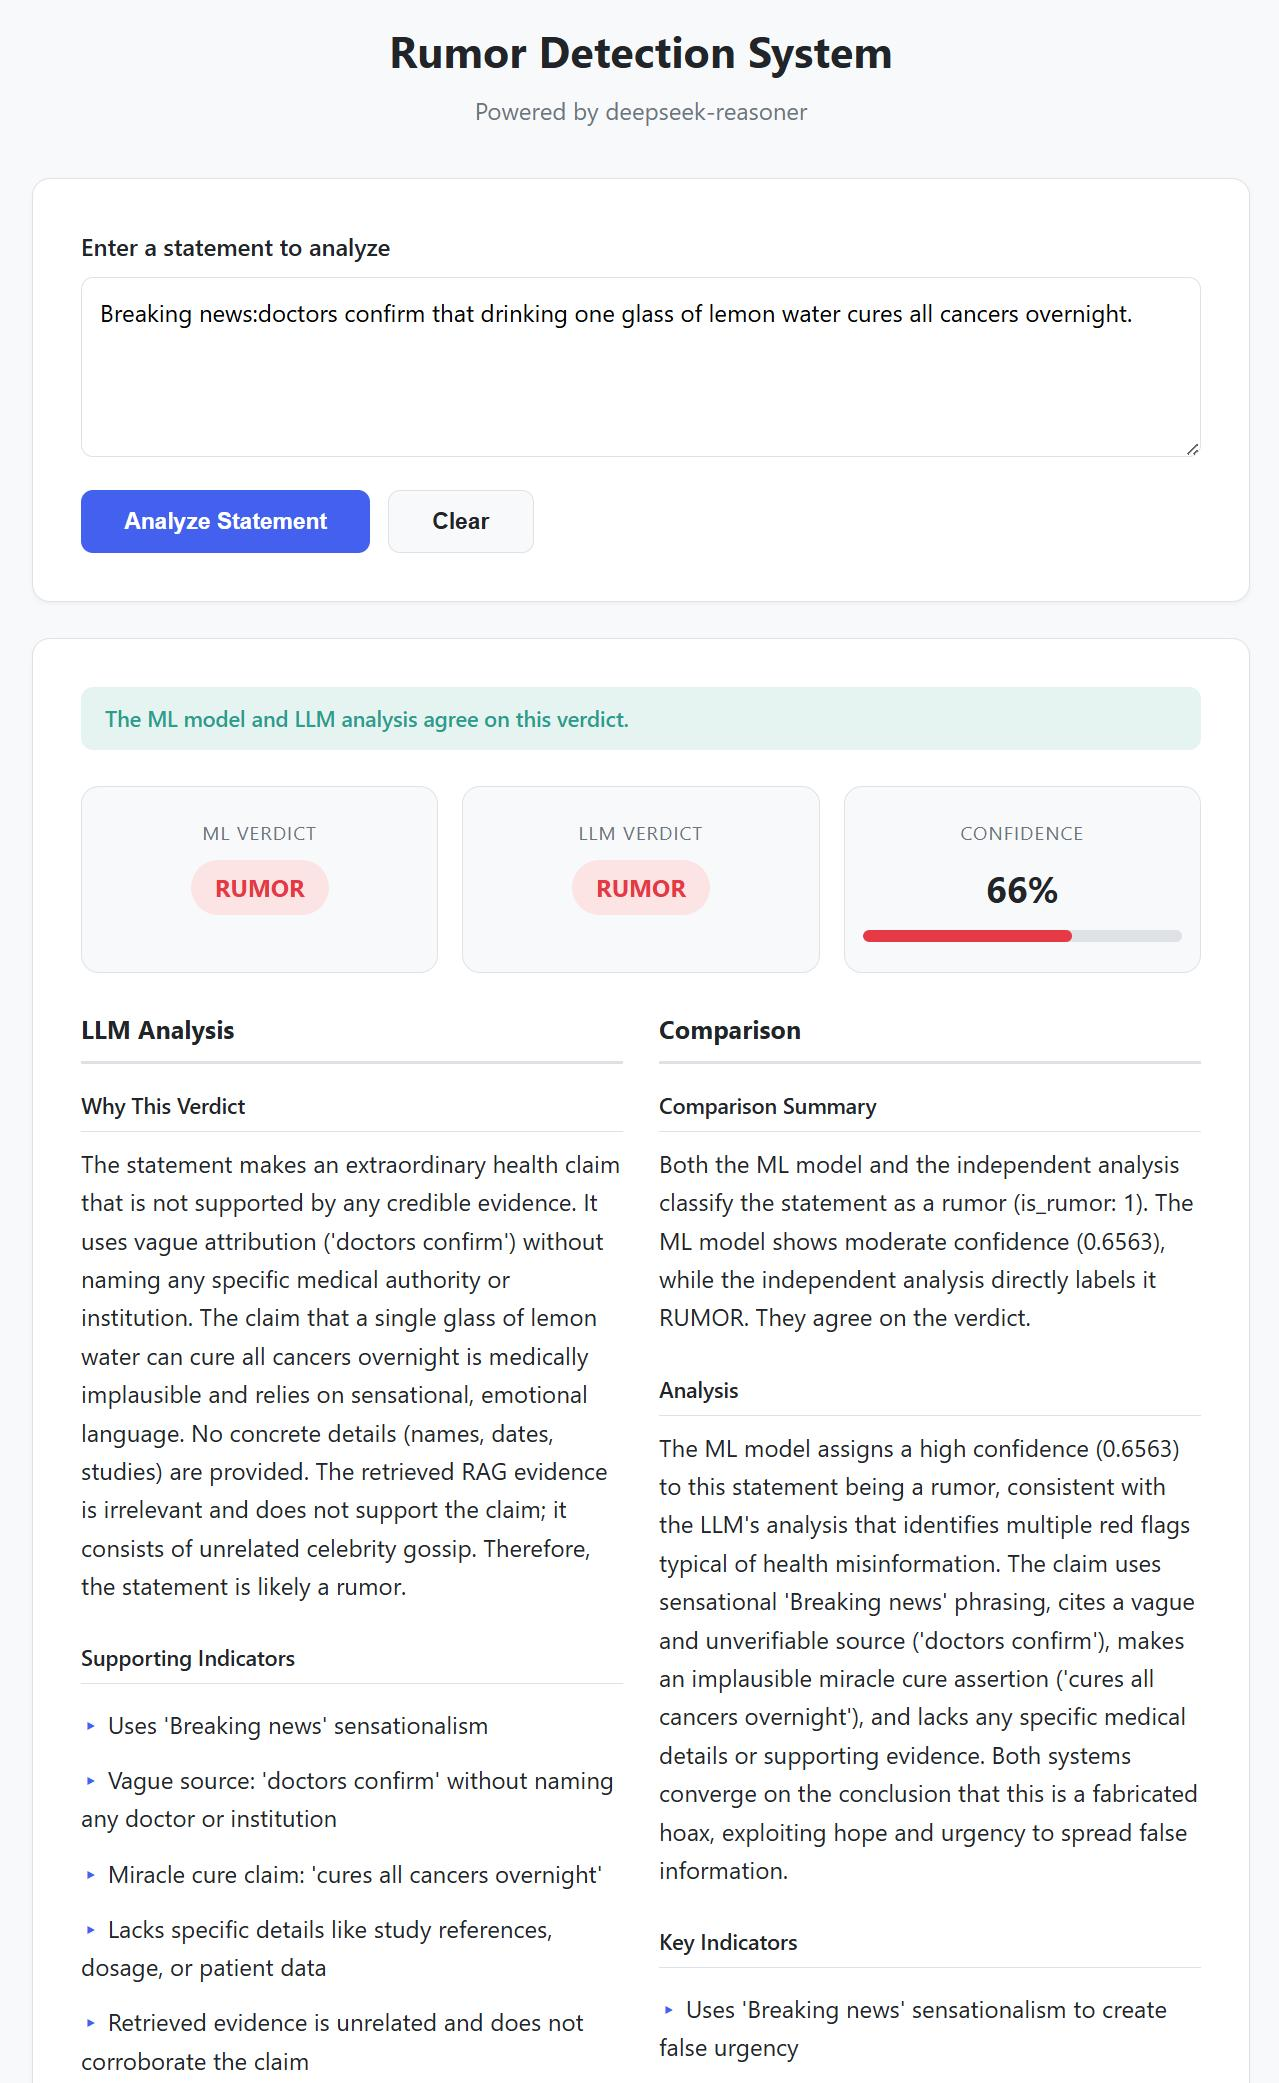
\includegraphics[width=0.74\textwidth]{img/frontend.png}
    \caption{前端页面展示示例}
    \label{fig:frontend}
\end{figure}

\subsubsection{LLM多阶段分析 —— \code{src/web/llm\_service.py}}

LLM分析模块是整个系统可解释性的核心，实现了三阶段提示工程管道：

LLM模块采用三阶段分析。第一阶段\code{judge\_statement()}结合输入文本和RAG证据进行独立判断，并输出结构化JSON；第二阶段\code{compare\_results()}比较ML与LLM结果是否一致；第三阶段\code{analyze\_root\_cause()}根据一致或分歧情况生成统一解释或根因分析。为了提高稳定性，\code{\_parse\_json()}对LLM返回结果进行容错解析，尽量从普通JSON、Markdown代码块或文本片段中提取结构化字段。

\subsubsection{FastAPI前端集成 —— \code{src/web/app.py}}

\code{src/web/app.py}以应用工厂组织完整流程，\code{/analyze}端点依次调用BERTweet分类、RAG检索、LLM独立判断、结果比较和根因分析，并将ML Verdict、LLM Verdict、Confidence、Reasoning、Comparison和RAG Evidence传入Jinja2模板。前端页面最终展示检测结果、解释文本和检索证据，如图\ref{fig:frontend}所示。

\subsection{检测结果分析}

本项目使用 \code{train.csv} 微调 BERTweet 模型，并在 \code{val.csv} 上验证。数据清洗后，训练集共 2832 条样本（非谣言 1596 条，谣言 1236 条），验证集共 400 条样本（非谣言 225 条，谣言 175 条），类别分布基本均衡，无明显长尾偏差。训练配置为学习率 $1\times10^{-5}$、batch size 32、最大训练 16 个 epoch，并以验证集 macro-F1 作为 early stopping 指标，patience=2，用连续两个 epoch 未提升触发停止。

实验结果显示，模型在第 5 个 epoch 取得最佳验证集表现：accuracy 为 0.8700，macro-F1 为 0.8688，验证集 loss 为 0.3696。早停机制在第 7 个 epoch 后触发，系统最终保存第 5 轮 macro-F1 最优的模型权重作为最终检测模型。

图3、图4与图5分别展示验证集 accuracy、macro-F1 以及训练/验证 loss 随 epoch 的变化。从曲线可见，accuracy 与 macro-F1 在前 5 轮持续上升，第 5 轮达到峰值后回落并趋于稳定；训练 loss 从 0.6735 下降到 0.1256，说明模型持续拟合训练集，而验证 loss 在第 5 轮降至 0.3696 后开始反弹（第 6 轮 0.4160，第 7 轮 0.4208），训练 loss 与验证 loss 的差距扩大，呈现典型过拟合特征。因此，采用 early stopping 能在性能峰值处保存模型，避免继续训练导致泛化能力下降。

\begin{figure}[H]
    \centering
    \begin{tikzpicture}
    \begin{axis}[
        width=0.85\textwidth,
        height=5.5cm,
        xlabel={Epoch},
        ylabel={Accuracy},
        xmin=0.5, xmax=7.5,
        ymin=0.68, ymax=0.90,
        xtick={1,2,3,4,5,6,7},
        ytick={0.70,0.75,0.80,0.85,0.90},
        legend pos=south east,
        legend cell align=left,
        grid=major,
        grid style={dashed, cgrey},
        mark=*,
        mark size=2.5pt,
        line width=1pt,
    ]
    \addplot[cyellow, mark=*] coordinates {
        (1, 0.7200) (2, 0.8150) (3, 0.8375)
        (4, 0.8525) (5, 0.8700) (6, 0.8625) (7, 0.8625)
    };
    \addplot[only marks, mark=*, mark size=4pt, cred] coordinates {(5, 0.8700)};
    \legend{验证集 Accuracy, 最佳点（Epoch 5）}
    \end{axis}
    \end{tikzpicture}
    \caption{验证集 Accuracy 随训练轮次变化曲线}
    \label{fig:accuracy_curve}
\end{figure}

\begin{figure}[H]
    \centering
    \begin{tikzpicture}
    \begin{axis}[
        width=0.85\textwidth,
        height=5.5cm,
        xlabel={Epoch},
        ylabel={Macro F1},
        xmin=0.5, xmax=7.5,
        ymin=0.67, ymax=0.89,
        xtick={1,2,3,4,5,6,7},
        ytick={0.70,0.75,0.80,0.85},
        legend pos=south east,
        legend cell align=left,
        grid=major,
        grid style={dashed, cgrey},
        mark=*,
        mark size=2.5pt,
        line width=1pt,
    ]
    \addplot[cyellow, mark=*] coordinates {
        (1, 0.7005) (2, 0.8116) (3, 0.8344)
        (4, 0.8490) (5, 0.8688) (6, 0.8610) (7, 0.8600)
    };
    \addplot[only marks, mark=*, mark size=4pt, cred] coordinates {(5, 0.8688)};
    \legend{验证集 Macro F1, 最佳点（Epoch 5）}
    \end{axis}
    \end{tikzpicture}
    \caption{验证集 Macro F1 随训练轮次变化曲线}
    \label{fig:f1_curve}
\end{figure}

\begin{figure}[H]
    \centering
    \begin{tikzpicture}
    \begin{axis}[
        width=0.85\textwidth,
        height=5.5cm,
        xlabel={Epoch},
        ylabel={Loss},
        xmin=0.5, xmax=7.5,
        ymin=0.08, ymax=0.72,
        xtick={1,2,3,4,5,6,7},
        legend pos=north east,
        legend cell align=left,
        grid=major,
        grid style={dashed, cgrey},
        mark=*,
        mark size=2.5pt,
        line width=1pt,
    ]
    \addplot[cyellow, mark=*] coordinates {
        (1, 0.6735) (2, 0.4859) (3, 0.3492)
        (4, 0.2823) (5, 0.2083) (6, 0.1642) (7, 0.1256)
    };
    \addplot[corange, mark=square*] coordinates {
        (1, 0.6208) (2, 0.4478) (3, 0.4199)
        (4, 0.3778) (5, 0.3696) (6, 0.4160) (7, 0.4208)
    };
    \addplot[only marks, mark=*, mark size=4pt, cred] coordinates {(5, 0.3696)};
    \legend{训练集 Loss, 验证集 Loss, 最佳点（Epoch 5）}
    \end{axis}
    \end{tikzpicture}
    \caption{训练集与验证集 Loss 随训练轮次变化曲线}
    \label{fig:loss_curve}
\end{figure}

最佳模型在验证集上的混淆矩阵如表1所示。模型对非谣言类（label 0）的精确率为0.9061、召回率为0.8578、F1为0.8813；对谣言类（label 1）的精确率为0.8289、召回率为0.8857、F1为0.8564。结果表明，模型对两类样本均有较稳定的识别能力，其中谣言类召回率较高，说明其更倾向于检出潜在谣言，符合谣言检测任务中降低漏检的需求。误判方面，32例非谣言被误判为谣言，20例谣言被误判为非谣言。

\begin{table}[H]
    \centering
    \begin{tabular}{|c|c|c|c|}
        \hline
        \multicolumn{2}{|c|}{} & \multicolumn{2}{c|}{\textbf{预测标签}} \\
        \cline{3-4}
        \multicolumn{2}{|c|}{} & \textbf{0（非谣言）} & \textbf{1（谣言）} \\
        \hline
        \multirow{2}{*}{\textbf{真实标签}} & \textbf{0（非谣言）} & 193 & 32 \\
        \cline{2-4}
        & \textbf{1（谣言）} & 20 & 155 \\
        \hline
    \end{tabular}
    \caption{最佳模型（Epoch 5）验证集混淆矩阵}
    \label{tab:confusion}
\end{table}

综上，微调后的BERTweet模型在较小规模数据集上取得了较为鲁棒的分类性能，accuracy与macro-F1均达到0.87左右，早停策略有效抑制了过拟合，模型在谣言检出率和非谣言精确率之间保持了合理的平衡。

\subsection{判断依据的分析}
本项目的判断依据主要由大语言模型生成，结合RAG检索证据提供辅助参考。
LLM会从可验证性、信源可信度、逻辑连贯性、情绪化语言和文本具体性等角度
生成解释。

当ML与LLM判断一致时，系统会生成统一解释；当两者判断不一致时，系统会提示分歧并分析原因。页面下方展示RAG Retrieved Evidence，包括证据来源、标签、距离和文本内容，增加判断过程的透明度。实验中也发现，RAG检索结果会受到数据库内容影响，因此本项目将RAG定位为解释增强模块，而不是最终分类依据。


\section{工作总结}
\subsection{收获与心得}
通过本项目，我们完整实践了一个AI应用系统的设计与实现过程，包括数据处理、预训练模型微调、模型评估、RAG检索增强、大语言模型API调用和前端展示。后期工程重构进一步统一了配置、依赖与命令行入口，并通过按领域拆分子包、延迟加载外部资产、兼容旧导入路径和补充回归测试，提高了系统的可维护性、可复现性与协作开发效率。项目加深了我们对Transformer文本分类模型、RAG检索机制和可解释AI系统设计的理解。

\subsection{问题与解决}
项目过程中主要遇到三个问题。
\begin{enumerate}
    \item 数据集规模较小，BERTweet型训练过多轮后容易过拟合。对此，我们采用验证集macro-F1作为早停指标，并保存最佳模型。
    \item 模型checkpoint、训练数据与RAG数据库体积较大，不适合直接提交到Git仓库。对此，我们将这些资产托管在Hugging Face，采用本地优先、缺失时自动下载并缓存的策略；RAG仍作为可选解释增强模块接入，保证外部资产不可用时主系统可以明确降级。
    \item LLM解释可能与小模型分类结果不一致。对此，我们设计了多阶段分析流程，将小模型判断、LLM判断和分歧分析分开展示。
\end{enumerate}

\subsection{分工与合作}
表\ref{tab:contributions}总结了我们小组成员的具体分工和贡献。

\begin{table}[H]
    \centering
    \begin{tabular}{|l|l|l|}
        \hline
        \textbf{成员} & \textbf{分工} & \textbf{贡献} \\
        \hline
        陈忠淳 & 项目统筹、小模型训练与评估 & GitHub 仓库管理、BERTweet微调与评估 \\
        沈润泽 & RAG模块开发 & 外部数据整理、ChromaDB 向量数据库构建、RAG独立运行测试 \\
        戴铭辰 & 前端与大模型调用 & FastAPI/Jinja2前端搭建与API调用、LLM三阶段分析流程设计 \\
        谢紫浩 & 报告与文档整理 & 实验报告撰写、README更新、RAG接入和最终运行检测\\
        \hline
    \end{tabular}
    \caption{小组成员分工与贡献}
    \label{tab:contributions}
\end{table}

\section{课程建议}
建议后续课程中可以提供更多关于模型部署、API调用、RAG接入和可解释性评估的知识讲解和应用示例，以帮助学生更好地完成从模型训练到系统实现的完整流程。增加可获取数据集的途径等，方便学生进一步探索。
\end{document}
